\section{\ix Design Approach}
\label{sec:design}

% We now present the fundamental design principles of a dataplane
% architecture designed to run untrusted, event-driven applicatxions,
% and designed to address the specific scalability challenges of
% today's web-scale applications.

The first three requirements of \S\ref{sec:motivation:challenges} --
high packet rate, microsecond latency, and connection scalability--
are not unique to web-scale applications.  These requirements have
been addressed in the design of middleboxes such as firewalls,
load-balancers, and software
routers~\cite{DBLP:journals/tocs/KohlerMCJK00,DBLP:conf/sosp/DobrescuEACFIKMR09};
by integrating the networking stack and the application into a single
\emph{dataplane}. The two remaining requirements -- resource
elasticity and protection -- are not addressed in middleboxes because
they are single-purpose systems, not exposed directly to users.

% As for the other two remaining aspects -- resource elasticity and
% security and protection --, middleboxes provide fewer insights: since
% each middlebox typically performs a single function, resource
% elasticity and proportionality is less of a direct concern.  They are
% traditionally deployed and maintained using an embedded paradigm in
% which the entire stack -- operating system, applications and utilities
% -- is packaged as single blob.  As such, the security and protection
% model is not directly exposed to users.

Dataplanes differ from traditional OS designs in two fundamental
ways. First, they are designed to \emph{run each packet to
  completion}. All network protocol and application processing for a
packet is done before moving on to the next packet.  In contrast, a
commodity OS decouples protocol processing from the application itself
in order to provide scheduling and flow control flexibility.  For
example, a commodity OS relies on device and soft interrupts to
context switch from application to protocol processing. Similarly, the
kernel's networking stack will generate a TCP \texttt{ACK} and slide
its receive window even when the application is not consuming data, up
to an extent. Second, dataplanes are designed to operate in a
\emph{flow-consistent, coherence-free} manner.  Network flows are
distributed into distinct queues via receive-side scaling
(RSS)~\cite{url:rss} and the common case packet processing requires no
synchronization or coherence traffic between cores.

% Flow-consistency distributes flows
% into distinct queues based on a L4-hash; this is routinely supported
% in network CPUs used in middleboxes (e.g., ~\cite{cavium-octeon}) as
% well as commodity NIC via Receive Side Scaling (RSS)~\cite{missing}.

Building upon the lessons from middleboxes, we design \ix to answer
the following question: {\it \ana{how} can the dataplane architecture be
  efficiently extended to support untrusted, event-driven applications
  and satisfy simultaneously the five requirements of
  \S\ref{sec:motivation:challenges}?}  The answer relies on the
following key design principles:


\myparagraph{Separation and protection of control and data plane:} 
% Software dataplanes are designed to operate on flows, not to
% provision resources or manage them in an elastic and proportional
% manner.
Our design separates the control function of the kernel, responsible
for resource configuration, provisioning, scheduling, and monitoring,
from the dataplane, which runs the networking stack and application
logic.  Like a conventional OS, the control plane multiplexes and
schedules resources among dataplanes, but in a coarse-grained manner
in space and time: cores are dedicated to applications until revoked,
memory is allocated at large page granularity of physical memory;
hardware queues are exclusively assigned to a single dataplane until
explicitly revoked.  The separation allows us to consider \george{double word?} radically
radically I/O APIs and implementations in the dataplane, while
retaining full compatibility with a modern OS like Linux.  Similar to
Exokernel~\cite{DBLP:conf/sosp/EnglerKO95}, each dataplane runs a
single application in a single address space.

 % of  using library operating systems~\cite{DBLP:conf/sosp/EnglerKO95}.

\myparagraph{Native zero-copy API with explicit flow control:} We do
not expose or emulate the POSIX API for networking.  Instead, the
dataplane and the application communicate asynchronously with each
other via messages stored in
memory~\cite{rizzo2012netmap,han2012megapipe}.  The API meets the
commutativity rule~\cite{DBLP:conf/sosp/ClementsKZMK13} and allows for
a true zero-copy operation in both directions. The dataplane and
application cooperatively manage the message buffer pool. Incoming
packets are mapped read-only into the application, which may hold onto
message buffers and return them to the dataplane at a later point.
The application sends to the dataplane scatter/gather lists of memory
locations for transmission but, since contents are not copied, the
application must keep the content immutable until the peer
acknowledges reception. The kernel implements all flow control
mechanisms and may trim transmission requests that exceed the
available size of the sliding window.  Essentially, the API directly,
but safely, exposes flow control to applications.


% \myparagraph{Explicit flow control:} The API supports a zero-copy,
% non-blocking API that directly, but safely, exposes flow control to
% applications. The application may send to the dataplane scatter/gather
% lists of memory locations for transmission.  The kernel trims requests
% that exceed the available size of the sliding window. As the contents
% are not copied, the application must further keep the content
% immutable until the peer later acknowledges reception.  Although the
% kernel implements all flow control mechanisms, it does not introduce
% additional buffering or abstraction mechanisms, allowing applications
% to make appropriate policy decisions.


\myparagraph{Run to completion with adaptive batching:} Our dataplane
runs to completion all pipeline stages needed to receive or transmit a
packet, interleaving protocol processing (kernel mode) and application
logic (user mode) as needed. Hence, there is no need for intermediate
buffering between pipeline stages or between the application logic and
the TCP/IP stack. Run to completion has been previously proposed to
address receive livelock within the OS~\cite{receivelivelock}. We
extend it to both kernel and user-level, which eliminates interrupts
and improves data locality throughout the common case packet
processing.

Batch processing minimizes instruction overheads and increases
instruction locality. Previous proposals batch only at the API level
in order to amortize system call
overhead~\cite{jeong2014mtcp,han2012megapipe,soares2010flexsc}. We
execute every pipeline stage on a small batch of packets or commands
to fully amortize instruction caching effects and the overhead of PCIe
transfers. To minimize the impact on latency, we perform adaptive
batching as follows: (i) we never wait to batch requests and batching
only occurs in the presence of congestion; (ii) we set an upper bound
on batches of 128 packets, a value experimentally determined to
effectively amortize startup overheads.


% Christos; this is essentially the other half of the "expose flow
% control to applications". oh well...
The combination of adaptive batch processing and zero copy means that
queues for incoming packets can build up only at the NIC edge, before
packets are processed by the dataplane. \ana{Emphasize that we are not
  wasting resources on packets that might have to be dropped; drop
  early at the NIC if can't handle.  Citation for Mogul and
  Ramakrishnan could go here.} The networking stack sends
acknowledgments to peers only as fast as the application can process
them. Any slowdown in the application processing rate quickly leads to
shrinking windows in peers. The dataplane also monitors queue depths
at the NIC edge and signals the control plane to allocate additional
resources for the dataplane (more hardware threads, increased clock
frequency), notify peers explicitly about congestion (e.g., via
ECN~\cite{ramakrishnan2001addition}), and make policy decisions for
congestion management (e.g., via
RED~\cite{DBLP:journals/ton/FloydJ93}).

% \myparagraph{Buffering at the NIC edge:} The consequence of adaptive
% batching is the buildup of queues at the NIC edge before the packets
% are processed by the dataplane.  Because of the dataplane's design,
% congestion occurs only at the NIC edge.  In effect, the NIC edge acts
% like the last-hop buffer in the network.  This has an additional
% benefit in terms of flow control, as the networking stack sends
% acknowledgments to peers only as fast as the application can process
% them.  Congestion in the NIC edge therefore leads to shrinking windows
% in peers, and flow control.


% Like switches and routers, the NIC edge can
% monitor queue depths to detect congestion, signal the control plane to
% allocate additional resources (more hardware threads, increase clock
% frequency) for the dataplane, notify explicitly flow sources of
% congestion (e.g., via ECN~\cite{ramakrishnan2001addition}), and finally make
% policy decisions when it is necessary to manage congestion (e.g., via RED~\cite{DBLP:journals/ton/FloydJ93}).

\begin{figure}
\begin{centering}
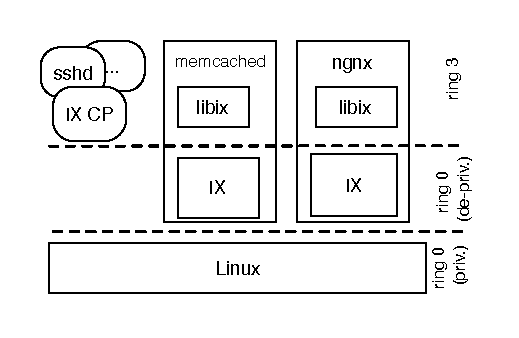
\includegraphics{figs/cp-dp.eps}
\centering\caption{Protection and separation in \ix.}
\label{fig:cp-dp}
\end{centering}
\end{figure}





\myparagraph{Flow consistent, coherence-free processing:} We use
multi-queue NICs with RSS support to provide flow-consistent hashing
of incoming traffic to distinct hardware queues. Each queue is served
by a single hardware thread all the way to the application layer,
eliminating the need for synchronization and cache coherence traffic
between cores. Similarly, memory management is organized in distinct
pools for each hardware thread. The absence of a socket layer
eliminates the issue of the shared file descriptor namespace in
multithreaded
applications~\cite{DBLP:conf/sosp/ClementsKZMK13}. Hence, our design
scales well with the increasing number of cores in modern servers. Our
approach does not restrict the memory model for
applications. Application logic can take advantage of coherent, shared
memory to exchange information and synchronize between cores.




